\documentclass[border=6pt]{standalone}
\usepackage{lmodern}
\usepackage{amsmath,amssymb}
\usepackage{tikz}
\usetikzlibrary{arrows.meta,shapes.geometric}
\begin{document}
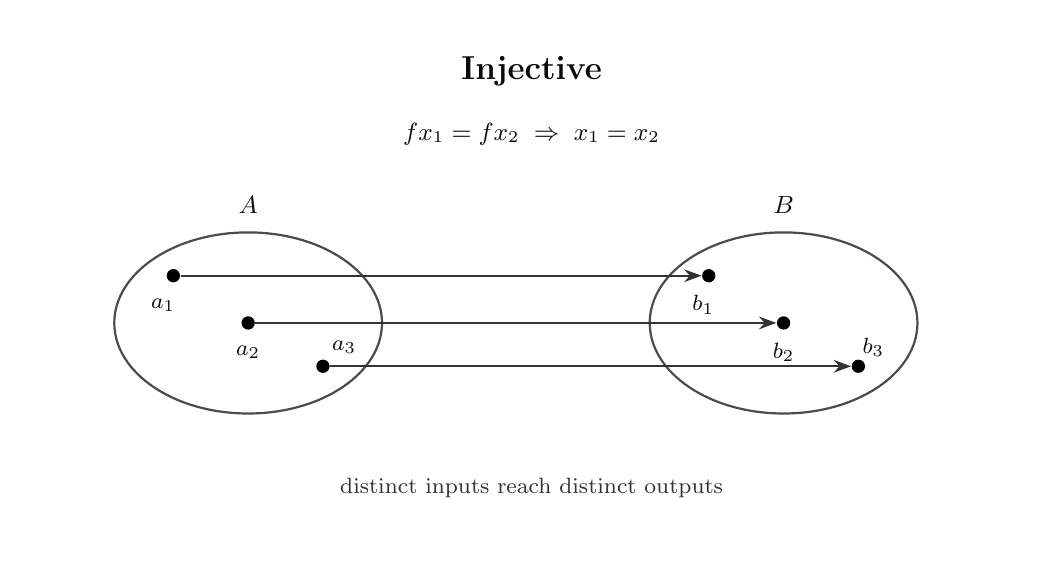
\begin{tikzpicture}[
  set/.style={draw=black!70, thick, ellipse, minimum width=3.4cm, minimum height=2.3cm},
  pt/.style={circle, fill=black, inner sep=1.7pt},
  map/.style={-{Stealth[length=2.2mm,width=1.6mm]}, thick, black!80},
  lab/.style={font=\footnotesize, text=black!94, fill=white, inner sep=1.2pt},
]
  \useasboundingbox (-0.4,-1.2) rectangle (12.2,5.3);
  \node[font=\large\bfseries, text=black!96] at (6,4.75) {Injective};
  \node[font=\small, text=black!96] at (6,3.95) {$f x_1 = f x_2 \;\Rightarrow\; x_1 = x_2$};
  \node[set] (A) at (2.4,1.55) {};
  \node[set] (B) at (9.2,1.55) {};
  \node[lab, font=\small] at (2.4,3.05) {$A$};
  \node[lab, font=\small] at (9.2,3.05) {$B$};
  \node[pt] (a1) at (1.45,2.15) {};
  \node[pt] (a2) at (2.40,1.55) {};
  \node[pt] (a3) at (3.35,1.00) {};
  \node[pt] (b1) at (8.25,2.15) {};
  \node[pt] (b2) at (9.20,1.55) {};
  \node[pt] (b3) at (10.15,1.00) {};
  \node[lab] at (1.32,1.78) {$a_1$};
  \node[lab] at (2.40,1.18) {$a_2$};
  \node[lab] at (3.62,1.24) {$a_3$};
  \node[lab] at (8.18,1.78) {$b_1$};
  \node[lab] at (9.20,1.18) {$b_2$};
  \node[lab] at (10.34,1.24) {$b_3$};
  \draw[map] (a1) -- (b1);
  \draw[map] (a2) -- (b2);
  \draw[map] (a3) -- (b3);
  \node[font=\footnotesize, text=black!80] at (6,-0.55) {distinct inputs reach distinct outputs};
\end{tikzpicture}
\end{document}
